\section{Formatowanie}
\label{sec:formatting}

Aby uniknąć nieporozumień dotyczących formatowania poniżej podsumowano najważniejsze informacje jego dotyczące. Czcionki tytułu, i~trzech poziomów zagnieżdżeń sekcji powinny odpowiednio przyjąć rozmiar 14, 12, 10, 10 punktów i~być pogrubione.

\subsection{Podział tekstu}
\label{subsec:textDivision}

W niniejszym przypadku, pierwszy akapit sekcji (niezależnie od poziomu ich zagnieżdżenia) występuje z pominięciem wcięcia.

Następujące po nim akapity powinny być wcięte.

\subsubsection{Poziomy sekcji}
\label{subsubsec:levels}

Zauważmy, że wyłącznie dwa poziomy sekcji są numerowane. Dalsze zagnieżdżenie skutkuje brakiem numeracji - wymagany sposób formatowania tekstu w~tym przypadku to wlewanie nagłówków w~tej samej linii, tak jak opisano w tej sekcji.

\paragraph{Granice zagnieżdżania}
\label{par:nestingLimits}

Pomimo, że szablon LLNCS Springer dopuszcza stosowanie czterech poziomów zagnieżdżenia, ostatni poziom najczęściej wpływa negatywnie na czytelność tekstu. Zainteresowany Czytelnik powinien stosować maksymalnie trzy opisywane poziomy, z~pominięciem poziomu zagnieżdżenia tej sekcji. Należy dążyć do rekomendowanej sytuacji, w~której stosowane są dwa poziomy zagnieżdżenia.

\subsubsection{Łamanie linii}
\label{subsubsec:linebreak}

Tekstu powinien być wyjustowany. Część wyrazów w~języku polskim (np. krótkie spójniki) nie może być stosowana na końcu linii. Aby tego uniknąć, należy zastosować skrypt porządkujący tekst lub korzystać ze znaku twardej spacji.

\subsubsection{Łamanie stron}
\label{subsubsec:pagebreak}

Dobrą praktyką, nie zawsze możliwą do realizacji, jest przejście do nowej strony na granicach akapitów i~w~taki sposób, aby w treści akapitu kończącego stronę nie było odwołania do ilustracji/tabeli znajdującego się na kolejnej. Należy również unikać kontynuacji niewielkiej części wątku na następnej stronie, szczególnie jeśli jest parzysta (czyli niewidoczna w~trybie czytania dwóch stron jednocześnie).

\subsubsection{Odstępy pionowe}
\label{subsubsec:verticalSpace}

Nadmierne odstępy pionowe utrudniają odbiór tekstu. Próba wdrożenia zasady łamania stron może wpłynąć na zwiększenie tych odstępów - należy unikać takiej sytuacji. Czytelnik jest zobowiązany do przeredagowania tekstu aby była możliwość umieszczenia jeszcze jednego akapitu na stronie, gdy doświadczy opisanego problemu.

\subsection{Uzupełnienia treści}
\label{subsec:additions}

Wśród popularnych obiektów urozmaicających treść są tabele i~rysunki. Rozpatrzmy oba przykłady (Tab. \ref{tab:styles}, Rys.). Zauważmy, że opis powinien znajdować się powyżej tabeli, ale poniżej rysunku. Należy zwrócić uwagę na dopasowanie rozmiaru obiektów do pozostałej treści strony.

\begin{table}
	\vspace{-4mm}
	\caption{
		Style wlewania tekstu.
	}
	\begin{center}
		\begin{tabular}{lll}
			\hline
			Typ & Przykład & Styl i~wielkość czcionki\\
			\hline
			Tytuł & {\Large\bfseries Instrukcja} & 14 punktów, pogrubiona\\
			Sekcja &  {\large\bfseries 1 Wprowadzenie} & 12 punktów, pogrubiona\\
			Podsekcja & {\bfseries 2.1 Podział tekstu} & 10 punktów, pogrubiona\\
			Paragraf & {\bfseries Poziomy sekcji} & 10 punktów, pogrubiona\\
			Zwykły tekst & Nadmierne odstępy pionowe & 10 punktów\\
			\hline
		\end{tabular}
	\end{center}
	\label{tab:styles}
	\vspace{-6mm}
\end{table}

\begin{figure}
	\begin{center}
		\vspace{-5mm}
		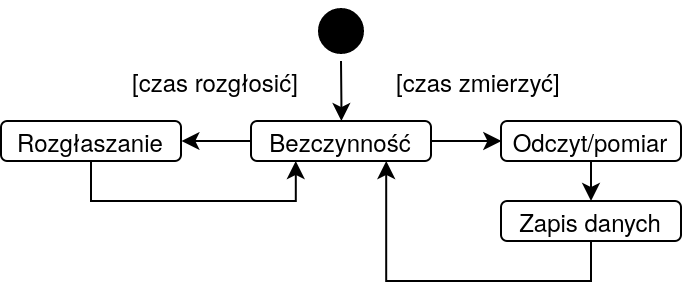
\includegraphics[width=8cm]{device-operation.png}
		\caption{
			Diagram stanów pracy beacona (model uproszczony). Po uruchomieniu i~konfiguracji urządzenie przechodzi w tryb zmniejszonego poboru energii. Operacje rozgłaszania i odczytu/pomiaru są najczęściej wykonywane okresowo.
		}
		\label{fig:devop}
		\vspace{-8mm}
	\end{center}
\end{figure}

Uzupełnienia treści powinny nawiązywać co najmniej do jednego akapitu sekcji. W~ten sposób Czytelnik jest w stanie poznać intencje autora dotyczące prezentacji obiektów urozmaicających w~artykule. Zbyt krótkie nawiązania mogą być przejawem niedokładności autora tekstu, a zbyt długie - utrudniać zrozumienie jego rozważań.
